\documentclass[14pt,aspectratio=169]{beamer}

% Assets
\usepackage[czech]{babel}				% Jazyk
\usepackage[a-2u]{pdfx}					% Kopírování z pdfka
\usepackage{tikz}						% Schémata automatů
\usepackage{csquotes}					% české uvozovky
\usepackage{enumerate}					% enumerate environment
\usepackage{indentfirst}
\usepackage{mathtools}
\usepackage{pifont}
\usepackage{xcolor}
\usepackage{enumitem,xcolor}
\usepackage{amsmath}
\usepackage[utf8]{inputenc}

\usepackage{listings}                   % Úryvky z kódu (C#)
\lstset{language=[Sharp]C, frame=lr}
% Beamer theme
\usetheme{Boadilla}
\setbeamertemplate{frame numbering}[fraction]
\usecolortheme[named=black]{structure}
\setbeamertemplate{navigation symbols}{}
\setbeamerfont{title}{series=\bfseries,parent=structure}
\setbeamerfont{frametitle}{series=\bfseries,parent=structure}
\usefonttheme[onlymath]{serif}
\urlstyle{same}

% Dark theme
\setbeamercolor{frametitle}{fg=white}
\setbeamercolor{title}{fg=white}
\setbeamercolor{background canvas}{bg=black}
\setbeamercolor{normal text}{fg=white}

\defbeamertemplate*{title page}{customized}[1][]
{ 
  \usebeamerfont*{title}\inserttitle\par
  \bigskip
  \usebeamerfont*{subtitle}\textit{\insertsubtitle}\par
  \bigskip \bigskip \bigskip \bigskip 
  \usebeamerfont{author}\insertauthor\par
  \usebeamerfont{institute}Kabinet \office\\\url{weber3@spsejecna.cz}\bigskip
}
% Enumerate
%\setlist[enumerate]{topsep=0pt,itemsep=-1ex,partopsep=1ex,parsep=1ex,label=(\arabic*)}

\MakeOuterQuote{"}

% Colors
\definecolor{lightblue}{HTML}{009AD4}
\definecolor{darkgreen}{HTML}{0D7103}
\definecolor{lightgreen}{HTML}{68FF00}
\definecolor{darkred}{HTML}{AF0B0B}
\definecolor{lightred}{HTML}{FF5100}
\definecolor{orange}{HTML}{FFE000}
\definecolor{codeblue}{HTML}{FF0055}
\definecolor{codegreen}{rgb}{0,0.6,0}
\definecolor{codegray}{rgb}{0.5,0.5,0.5}
\definecolor{codebeige}{HTML}{D4A000}
\definecolor{backcolour}{rgb}{0.95,0.95,0.92}

\newcommand{\markred}[1]{\textcolor{lightred}{#1}}
\newcommand{\markgreen}[1]{\textcolor{lightgreen}{#1}}
\newcommand{\markorange}[1]{\textcolor{orange}{#1}}
\newcommand{\markblue}[1]{\textcolor{lightblue}{#1}}

% Inline images
\newcommand{\inlineimgscale}{1.1}

% X and check mark
\newcommand{\cmark}{\markgreen{\ding{51}}}
\newcommand{\xmark}{\markred{\ding{55}}}

% Redefinions
\renewcommand{\implies}{\Rightarrow}
\renewcommand{\impliedby}{\Leftarrow}

% Math
\newcommand{\R}{\mathbb{R}}
\newcommand{\C}{\mathbb{C}}
\newcommand{\N}{\mathbb{N}}
\newcommand{\Z}{\mathbb{Z}}
\newcommand{\Q}{\mathbb{Q}}

% Code
\lstdefinestyle{clang}{
    basicstyle=\small\ttfamily\color{white},
    language=C,
    keywordstyle=\color{codeblue},
    commentstyle=\color{codegreen},
    numberstyle=\tiny\color{codegray},
    stringstyle=\color{codebeige},
    breakatwhitespace=false,
    breaklines=true,
    captionpos=b,
    keepspaces=true,
    numbersep=5pt,
    showspaces=false,
    showstringspaces=false,
    showtabs=false,
    morekeywords={void,int,double,float,unsigned,if,else,\#include}
    tabsize=0.5
}
\lstset{escapeinside={(*}{*)},style=clang}

\newcommand{\hlcode}[1]{\colorbox{red}{#1}}

% Title page
\title{Funkce v C}
\subtitle{Informační a komunikační technologie}
\author{David Weber}
\def\office{K13}
\def\email{weber3@spsejecna.cz}

\begin{document}

    % Itemize
    \setlist[itemize]{label=\textcolor{white}{\textbullet}}

    % Slides
    \begin{frame}
        \titlepage
    \end{frame}

    \begin{frame}[t,fragile]{Příklad na úvod}
        \begin{lstlisting}
// Print array
for (int i = 0; i < size; i++) {
    printf("%d ", arr[i]);
}
printf("\n");
// Square array elements
for (int i = 0; i < size; i++) {
    arr[i] *= arr[i];
}
// Print array
for (int i = 0; i < size; i++) {
    printf("%d ", arr[i]);
}
        \end{lstlisting}
    \end{frame}

    \begin{frame}[t,fragile]{V čem je problém?}
        \begin{itemize}
            \item Kód je funkční, ale část pro výpis pole je zde uvedena \textbf{dvakrát}.
            \begin{lstlisting}
for (int i = 0; i < size; i++) {
    printf("%d ", arr[i]);
}
            \end{lstlisting}
            \item \markred{Opakující kód je nepraktický} \xmark
            \begin{itemize}
                \item budeme-li chtít změnit nějakou jeho část, musíme změnu provést všude
            \end{itemize}
            \item \markgreen{Použijeme funkci} \cmark
        \end{itemize}
    \end{frame}

    \begin{frame}[t]{Co je to funkce?}
        \begin{itemize}
            \item Obecně se jedná o část programu, kterou je možné opakovaně ``vyvolat'' v různých místech programu.
            \item Motivace pro použití:
            \begin{itemize}
                \item odstranění opakování kódu v programu,
                \item rozklad složitých problémů na jednodušší,
                \item znovupoužití v jiných programech, např. formou knihoven (to až ve druháku \emoji{shushing-face}).
            \end{itemize}
        \end{itemize}
    \end{frame}

    \begin{frame}[t,fragile]{Struktura funkce}
        \begin{lstlisting}
navratovy_typ jmeno(parametry) {
    <implementace>
}
        \end{lstlisting}
        \begin{itemize}
            \item U funkce je třeba specifikovat:
            \begin{itemize}
                \item návratový datový typ,
                \item jméno (identifikátor),
                \item parametry,
                \item tělo (implementace).
            \end{itemize}
            \item Funkce uvádíme mimo tělo funkce \texttt{main}.
        \end{itemize}
    \end{frame}

    \begin{frame}[t,fragile]{Funkce bez parametrů}
        \begin{itemize}
            \item Nejjednodušší typ funkce.
            \item Klíčové slovo \markblue{\texttt{void}} (prázdný datový typ), do závorek \texttt{(\markblue{void})} nebo nechat prázdné, tj. \texttt{()}
            \begin{lstlisting}
void greet(void) {
    printf("Hello World!");
}
            \end{lstlisting}
            \item \textbf{Doporučení:} funkci uvádějte nad \texttt{main}!
            \item Samotná definice funkce nic nedělá $\implies$ \markorange{je třeba ji tzv. \textbf{zavolat}.}
        \end{itemize}
    \end{frame}

    \begin{frame}[t,fragile]{Volání funkce}
        \begin{itemize}
            \item Je třeba specifikovat, kde v programu se má daná funkce provést.
            \begin{lstlisting}
void greet(void) {
    printf("Hello World!");
}
            
int main(void) {

    greet();    // Prints out "Hello World!"

    return 0;
}
            \end{lstlisting}
        \end{itemize}
    \end{frame}

    \begin{frame}[t,fragile]{Funkce s parametry}
        \begin{itemize}
            \item Často budeme chtít činnost funkce zobecnit (výstup funkce bude na něčem záviset).
            \item $\implies$ k tomu použijeme tzv. \textbf{parametry}.
            \item Do kulatých závorek \texttt{()} uvádíme výčet parametrů (jejich datový typ a název), které funkce přijímá.
            \begin{lstlisting}
void fce(<datovy_typ> var1, <datovy_typ> var2, ...) {
    ...
}
            \end{lstlisting}
        \end{itemize}
    \end{frame}

    \begin{frame}[t,fragile]{Příklad I (funkce s parametrem)}
        \begin{lstlisting}
void square(float x) {
    printf("Druha mocnina x je %g", x*x);
}

int main(void) {

    float input;
    scanf("%f", &input);

    square(input);
    
    return 0;
}
        \end{lstlisting}
    \end{frame}

    \begin{frame}[t,fragile]{Příklad II (funkce s více parametry)}
        Funkce pro výpočet aritmetického průměru celých čísel $a,\,b\in\Z$:
        \begin{lstlisting}
void average(int a, int b) {
    float avg = (a + b) / 2;
    printf("%g", avg);
}

int main(void) {
    float input1, input2;
    scanf("%d %d", &input1, &input2);

    average(input1, input2);
    
    return 0;
}
        \end{lstlisting}
    \end{frame}

    \begin{frame}{Úloha I}
        Předělejte program pro výpis faktoriálu, tj.
        \begin{equation*}
            n!=n(n-1)(n-2)\cdots 2\cdot 1,
        \end{equation*}
        do funkce. (Viz domácí úkol \emoji{slightly-smiling-face})
    \end{frame}

    \begin{frame}[t,fragile]{Funkce s návratovou hodnotou I}
        \begin{itemize}
            \item \textbf{Problém:} s hodnotou, kterou funkce vypočte, nemůžeme dále pracovat (pouze ji na konci vypisujeme).
            \item Např. u funkcí \texttt{pow}, \texttt{sqrt}, \dots (viz knihovna \textbf{math}) jsme mohli s vypočtenou hodnotou dále počítat
            \begin{lstlisting}
float hypotenuse = sqrt(pow(x, 2) + pow(y, 2));
printf("%f", hypotenuse);
            \end{lstlisting}
            \item $\implies$ \markgreen{využijeme tzv. \textbf{návratovou hodnotu}.}
        \end{itemize}
    \end{frame}

    \begin{frame}[t,fragile]{Funkce s návratovou hodnotou II}
        \begin{itemize}
            \item Klíčové slovo \markblue{\texttt{return}}.
            \item Před názvem funkce musíme dále uvést datový typ návratové hodnoty funkce.
            \item Např. funkce pro výpočet faktoriálu vracející výsledek:
            \begin{lstlisting}
int factorial(int n) {
    int fact = 1;
    for (int i = 1; i <= n; i++) {
        fact *= i;
    }
    return fact;
}
            \end{lstlisting}
        \end{itemize}
    \end{frame}

    \begin{frame}{Úloha II}
        Napište vlastní funkci pro výpočet $n$-té mocniny čísla $x\in\R$. Funkce bude přijímat parametry $x,\,n$ a bude vracet $x^n$. Nesmíte použít funkci \texttt{pow}. \emoji{upside-down-face}
    \end{frame}

    \begin{frame}[t]{Co se děje uvnitř?}
        \begin{itemize}
            \item Při volání funkce program vykoná její kód a následně se vrátí do místa jejího volání, odkud pokračuje.
            \item \markred{$\implies$ jak ale ví, odkud má pokračovat? Jaké byly stavy proměnných při volání?}
        \end{itemize}
    \end{frame}

    \begin{frame}[t,fragile]{Příklad}
        \begin{columns}[onlytextwidth]
            \begin{column}{0.55\textwidth}
                \begin{itemize}
                    \item Program začne ve funkci \texttt{main}, kde inicializuje proměnné \texttt{a} a \texttt{b},
                    \item při zavolání funkce \texttt{mult} je navrácena hodnota $x\cdot y$ a vrátíme se zpět do místa volání (tj. do funkce \texttt{main}),
                    \item \markorange{$\implies$ je třeba vědět, do které části kódu se přesunout!} \markgreen{$\implies$ návratová adresa}.
                \end{itemize}
            \end{column}
            
            \begin{column}{0.41\textwidth}
                \begin{lstlisting}
int mult(int x, int y) {
    return x*y;
}
int main(void) {
    int a = 10;
    int b = 47;
    printf("%d", mult(a, b));
    return 0;
}
                \end{lstlisting}
            \end{column}
        \end{columns}
        
    \end{frame}

    \begin{frame}[t]{Zásobník}
        \begin{itemize}
            \item \textbf{Návratová adresa} -- adresa v paměti, odkud má program pokračovat po skončení volané funkce.
            \item Při volání funkce a návratu z ní se využívá tzv. \textbf{zásobník} (angl. \emph{stack}).
            \item Do něj se ukládá (mimo jiné) \textbf{při volání funkce} \emph{návratová adresa}, \emph{předávané parametry \textbf{volané} funkce}.
            \item Dále jsou zde ukládány i \emph{hodnoty lokálních proměnných}.
        \end{itemize}
    \end{frame}

    \begin{frame}[t]{Rozdělení paměti}
        \begin{columns}[onlytextwidth,T]
            \column{\dimexpr\linewidth-30mm-3mm}
            \begin{itemize}
                \item \textbf{Kód programu} -- zkompilovaný (strojový) kód programu
                \item \textbf{Statická data} -- mají svou velikost přesně a neměně určenou v okamžiku překladu zdrojového textu (globální proměnné)
                \item \textbf{Zásobník} -- lokální proměnné, argumenty funkcí, návratová hodnota funkce, \emph{návratová adresa}
                \item \textbf{Halda} -- dynamická paměť, alokována za běhu programu (např. v případě pole)
            \end{itemize}
      
            \column{30mm}
            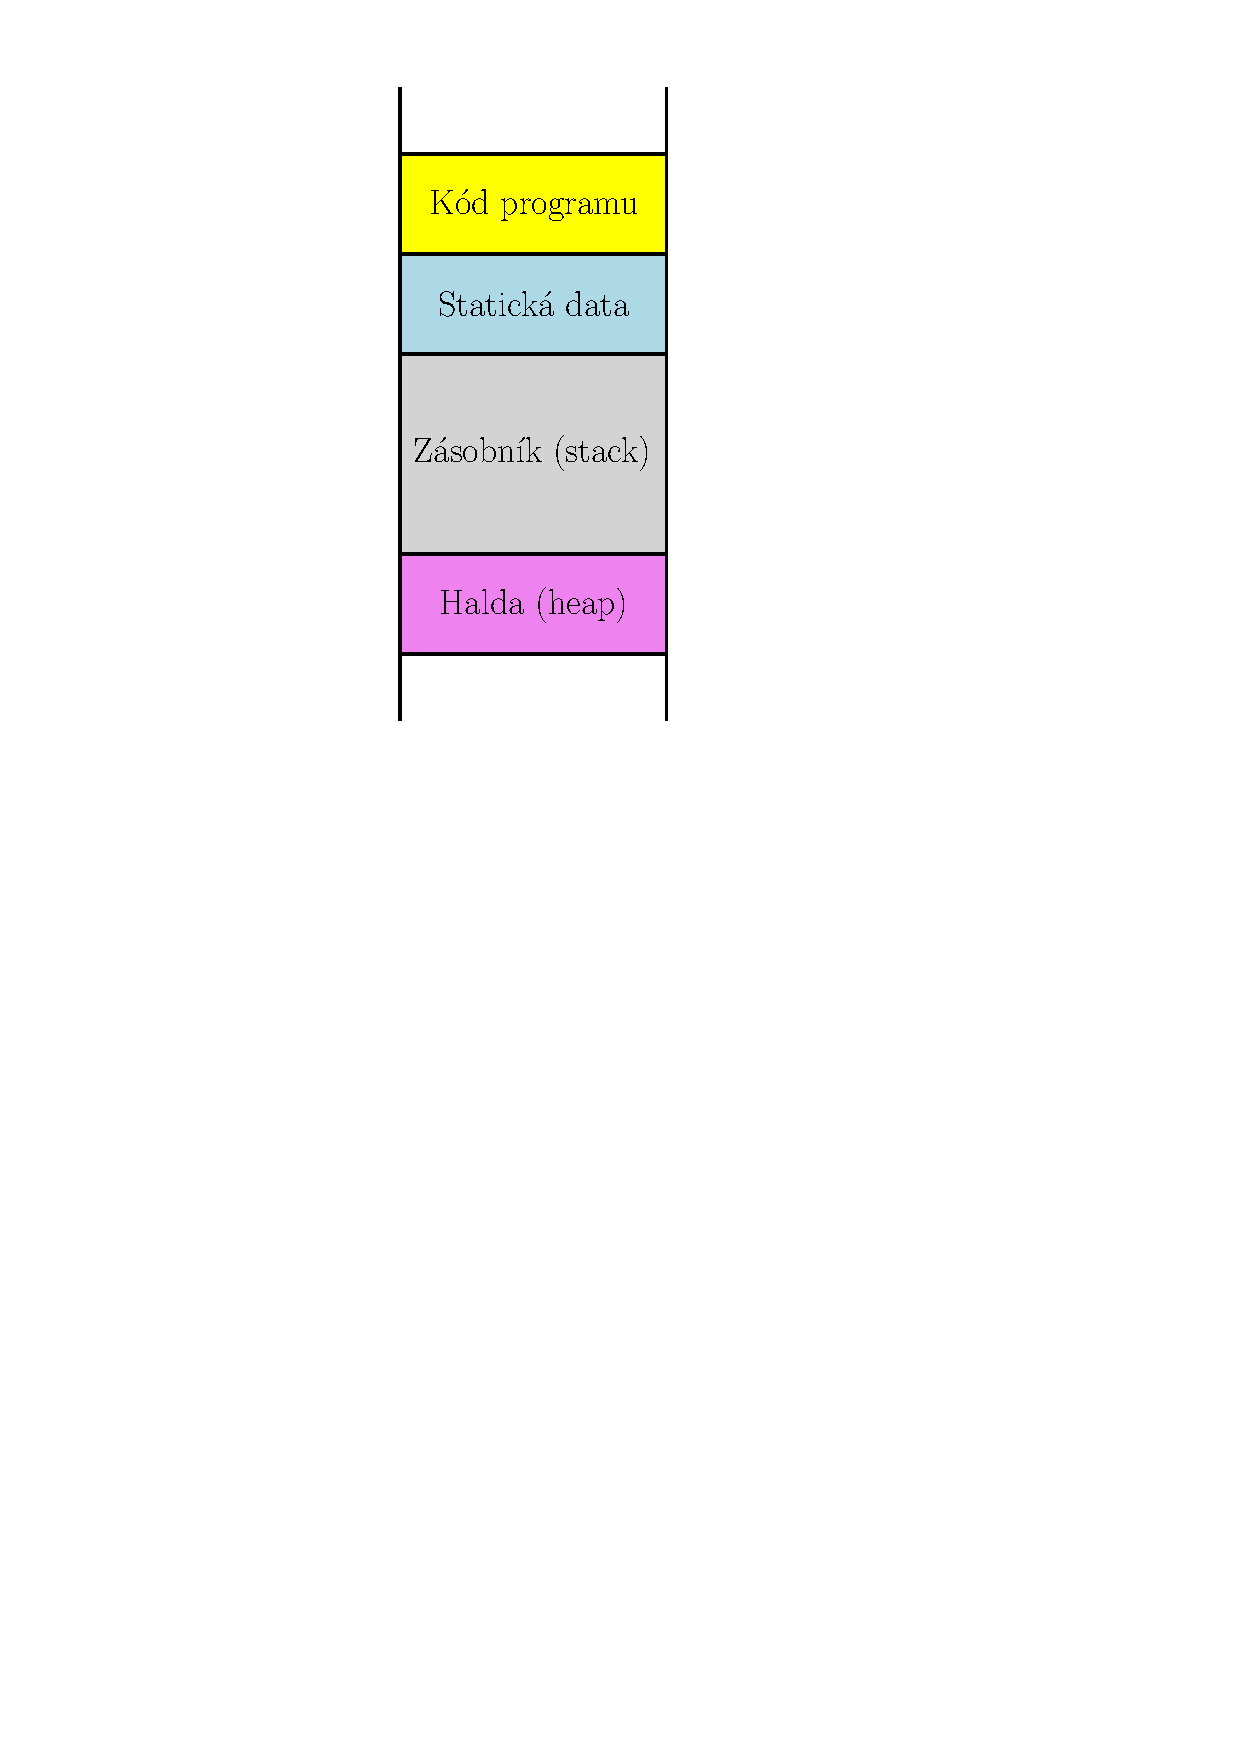
\includegraphics[width=30mm]{images/program_v_pameti.pdf}
        \end{columns}
    \end{frame}

    \begin{frame}{Otázky?}
        \begin{figure}
            \centering
            
\includegraphics[scale=.4]{images/discussion_inverted.png}
        \end{figure}
    \end{frame}

\end{document}